\documentclass{standalone}
\usepackage{tikz}
\usetikzlibrary{patterns, positioning}
\usepackage[sfdefault]{ClearSans} %% option 'sfdefault' activates Clear Sans as the default text font
\usepackage[T1]{fontenc}

\begin{document}
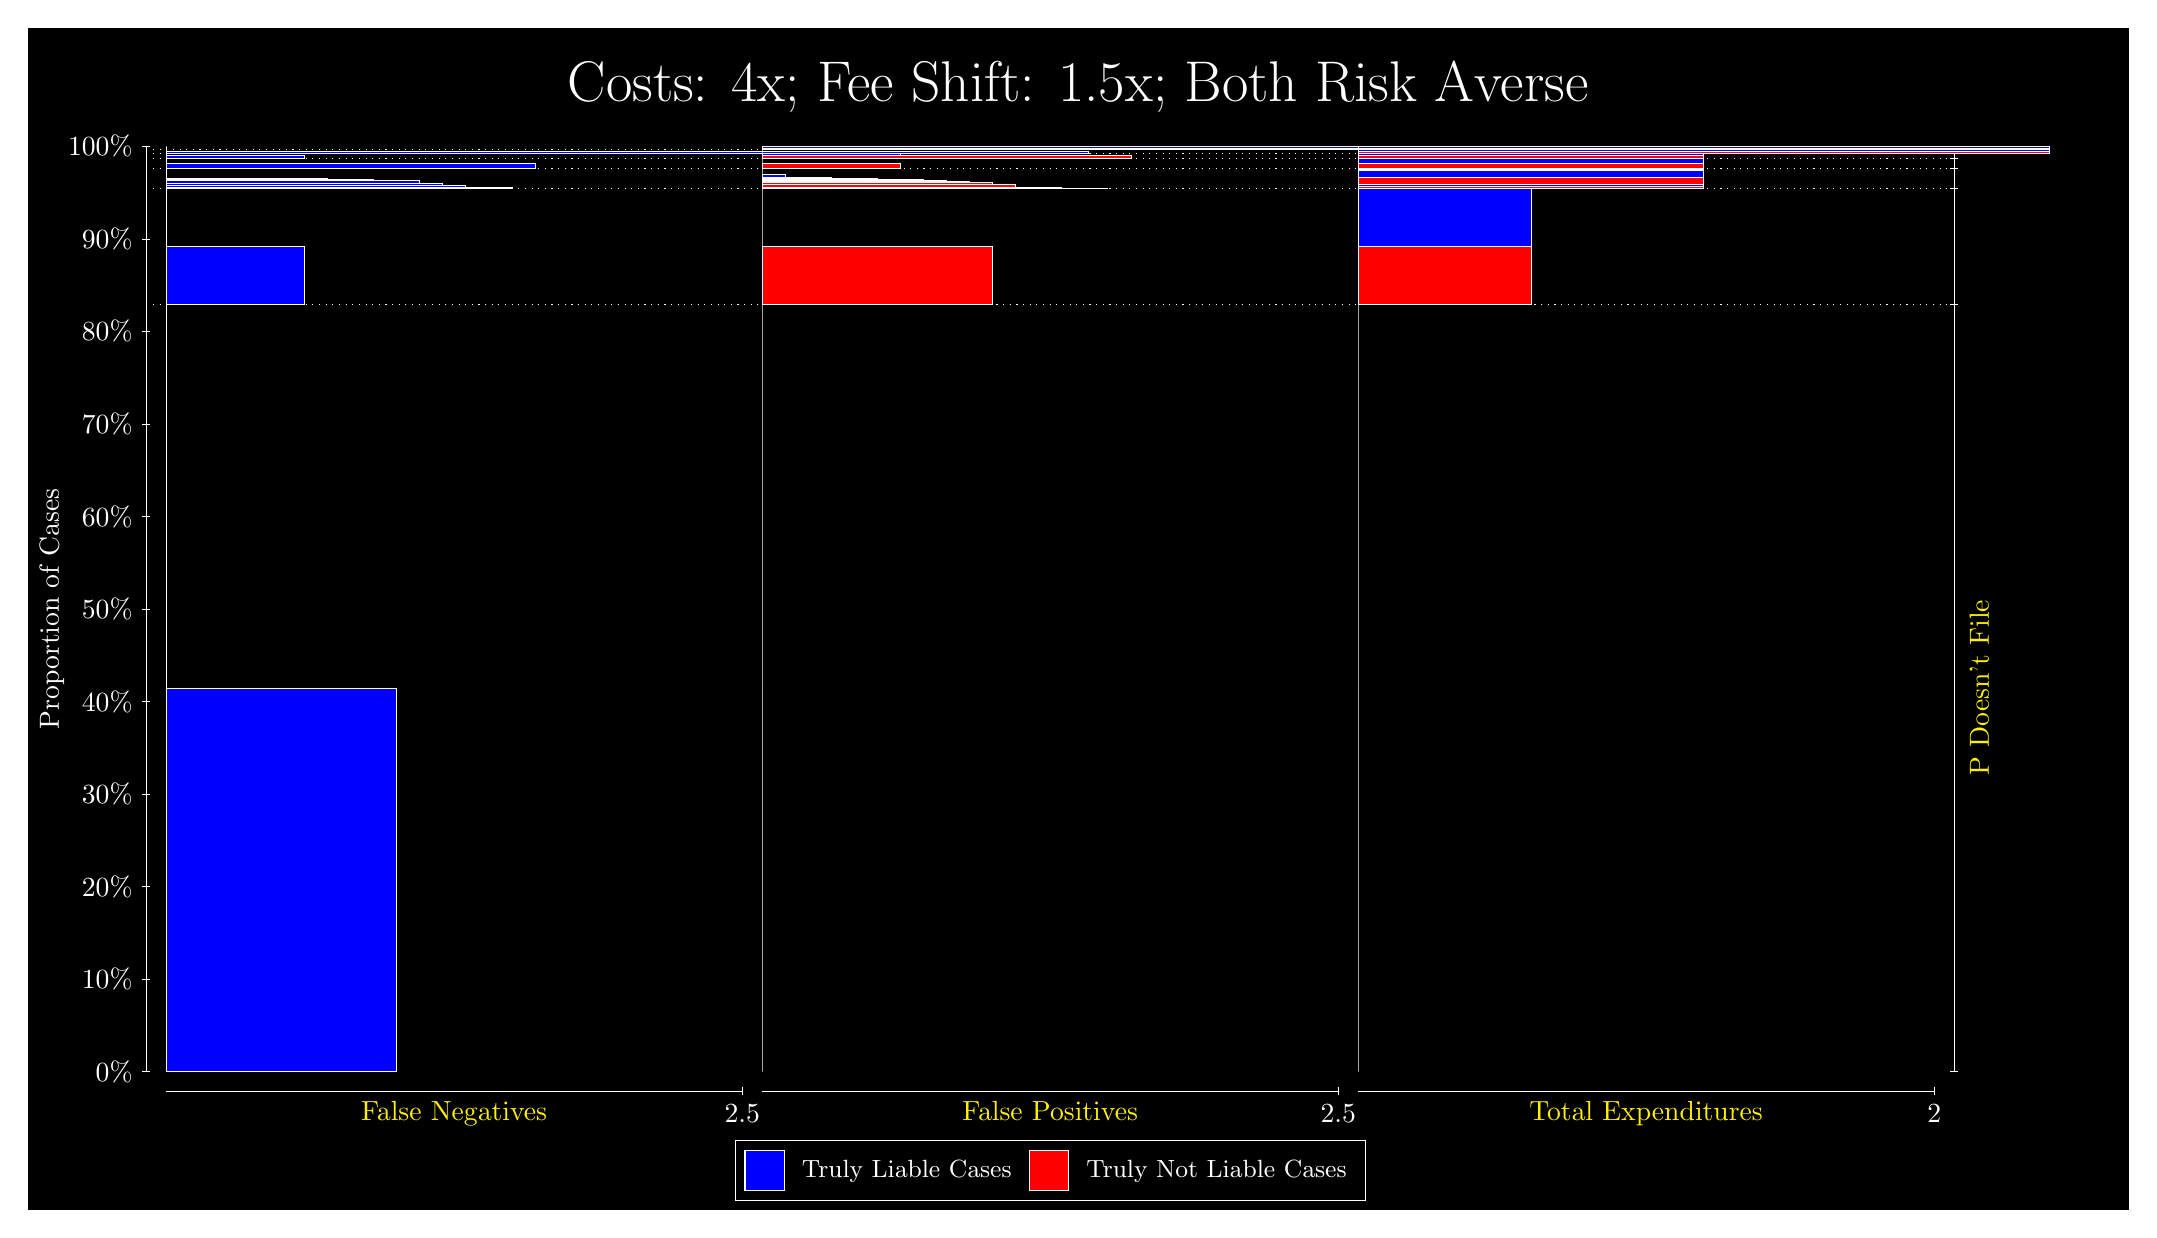
\begin{tikzpicture}
\draw[fill=black] (0,0) rectangle (26.667,15);
\draw[text=white] (0,13.5) rectangle (26.667,15) node[midway] {\huge Costs: 4x; Fee Shift: 1.5x; Both Risk Averse};
\draw[white, very thin] (1.5,1.75) -- (1.5,13.5);
\node[rotate=90, text=white, anchor=center] at (0.3, 7.625) {Proportion of Cases};
\draw[white, very thin] (1.45,1.75) -- (1.55,1.75);
\node[text=white, anchor=east] at (1.45, 1.75) {0\%};
\draw[white, very thin] (1.45,2.925) -- (1.55,2.925);
\node[text=white, anchor=east] at (1.45, 2.925) {10\%};
\draw[white, very thin] (1.45,4.1) -- (1.55,4.1);
\node[text=white, anchor=east] at (1.45, 4.1) {20\%};
\draw[white, very thin] (1.45,5.275) -- (1.55,5.275);
\node[text=white, anchor=east] at (1.45, 5.275) {30\%};
\draw[white, very thin] (1.45,6.45) -- (1.55,6.45);
\node[text=white, anchor=east] at (1.45, 6.45) {40\%};
\draw[white, very thin] (1.45,7.625) -- (1.55,7.625);
\node[text=white, anchor=east] at (1.45, 7.625) {50\%};
\draw[white, very thin] (1.45,8.8) -- (1.55,8.8);
\node[text=white, anchor=east] at (1.45, 8.8) {60\%};
\draw[white, very thin] (1.45,9.975) -- (1.55,9.975);
\node[text=white, anchor=east] at (1.45, 9.975) {70\%};
\draw[white, very thin] (1.45,11.15) -- (1.55,11.15);
\node[text=white, anchor=east] at (1.45, 11.15) {80\%};
\draw[white, very thin] (1.45,12.325) -- (1.55,12.325);
\node[text=white, anchor=east] at (1.45, 12.325) {90\%};
\draw[white, very thin] (1.45,13.5) -- (1.55,13.5);
\node[text=white, anchor=east] at (1.45, 13.5) {100\%};

\draw[white, very thin] (24.457,1.75) -- (24.457,13.5);
\draw[white, very thin] (24.407,1.75) -- (24.507,1.75);
\node[anchor=west] at (24.407, 1.75) {};
\draw[white, very thin] (24.407,11.495) -- (24.507,11.495);
\node[anchor=west] at (24.407, 11.495) {};
\draw[white, very thin] (24.407,12.961) -- (24.507,12.961);
\node[anchor=west] at (24.407, 12.961) {};
\draw[white, very thin] (24.407,13.215) -- (24.507,13.215);
\node[anchor=west] at (24.407, 13.215) {};
\draw[white, very thin] (24.407,13.349) -- (24.507,13.349);
\node[anchor=west] at (24.407, 13.349) {};
\draw[white, very thin] (24.407,13.413) -- (24.507,13.413);
\node[anchor=west] at (24.407, 13.413) {};
\draw[white, very thin] (24.407,13.462) -- (24.507,13.462);
\node[anchor=west] at (24.407, 13.462) {};
\draw[white, very thin] (24.407,13.5) -- (24.507,13.5);
\node[anchor=west] at (24.407, 13.5) {};

\draw[white, very thin, fill=blue] (1.75,1.75) rectangle (4.6775,6.6227);
\draw[white, very thin, fill=red] (1.75,6.6227) rectangle (1.75,11.495);
\draw[white, very thin, fill=blue] (1.75,11.495) rectangle (3.5065,12.231);
\draw[white, very thin, fill=red] (1.75,12.231) rectangle (1.75,12.961);
\draw[white, very thin, fill=blue] (1.75,12.961) rectangle (6.1413,12.977);
\draw[white, very thin, fill=blue] (1.75,12.977) rectangle (5.8486,12.984);
\draw[white, very thin, fill=blue] (1.75,12.984) rectangle (5.5558,13.01);
\draw[white, very thin, fill=blue] (1.75,13.01) rectangle (5.2631,13.036);
\draw[white, very thin, fill=blue] (1.75,13.036) rectangle (4.9703,13.064);
\draw[white, very thin, fill=blue] (1.75,13.064) rectangle (4.6775,13.074);
\draw[white, very thin, fill=blue] (1.75,13.074) rectangle (4.3848,13.082);
\draw[white, very thin, fill=blue] (1.75,13.082) rectangle (4.092,13.085);
\draw[white, very thin, fill=blue] (1.75,13.085) rectangle (3.7993,13.089);
\draw[white, very thin, fill=red] (1.75,13.089) rectangle (1.75,13.215);
\draw[white, very thin, fill=blue] (1.75,13.215) rectangle (6.4341,13.279);
\draw[white, very thin, fill=red] (1.75,13.279) rectangle (1.75,13.349);
\draw[white, very thin, fill=blue] (1.75,13.349) rectangle (3.5065,13.382);
\draw[white, very thin, fill=red] (1.75,13.382) rectangle (1.75,13.413);
\draw[white, very thin, fill=blue] (1.75,13.413) rectangle (13.46,13.431);
\draw[white, very thin, fill=red] (1.75,13.431) rectangle (1.75,13.462);
\draw[white, very thin, fill=red] (1.75,13.462) rectangle (1.75,13.477);
\draw[white, very thin, fill=blue] (1.75,13.477) rectangle (1.75,13.5);
\draw[white, very thin, fill=red] (9.3189,1.75) rectangle (9.3189,6.6227);
\draw[white, very thin, fill=blue] (9.3189,6.6227) rectangle (9.3189,11.495);
\draw[white, very thin, fill=red] (9.3189,11.495) rectangle (12.246,12.226);
\draw[white, very thin, fill=blue] (9.3189,12.226) rectangle (9.3189,12.961);
\draw[white, very thin, fill=red] (9.3189,12.961) rectangle (13.71,12.965);
\draw[white, very thin, fill=red] (9.3189,12.965) rectangle (13.417,12.968);
\draw[white, very thin, fill=red] (9.3189,12.968) rectangle (13.125,12.976);
\draw[white, very thin, fill=red] (9.3189,12.976) rectangle (12.832,12.986);
\draw[white, very thin, fill=red] (9.3189,12.986) rectangle (12.539,13.013);
\draw[white, very thin, fill=red] (9.3189,13.013) rectangle (12.246,13.038);
\draw[white, very thin, fill=red] (9.3189,13.038) rectangle (11.954,13.062);
\draw[white, very thin, fill=red] (9.3189,13.062) rectangle (11.661,13.068);
\draw[white, very thin, fill=red] (9.3189,13.068) rectangle (11.368,13.087);
\draw[white, very thin, fill=blue] (9.3189,13.087) rectangle (10.783,13.09);
\draw[white, very thin, fill=blue] (9.3189,13.09) rectangle (10.49,13.094);
\draw[white, very thin, fill=blue] (9.3189,13.094) rectangle (10.197,13.102);
\draw[white, very thin, fill=blue] (9.3189,13.102) rectangle (9.9044,13.112);
\draw[white, very thin, fill=blue] (9.3189,13.112) rectangle (9.6116,13.139);
\draw[white, very thin, fill=blue] (9.3189,13.139) rectangle (9.3189,13.215);
\draw[white, very thin, fill=red] (9.3189,13.215) rectangle (11.075,13.285);
\draw[white, very thin, fill=blue] (9.3189,13.285) rectangle (9.3189,13.349);
\draw[white, very thin, fill=red] (9.3189,13.349) rectangle (14.003,13.38);
\draw[white, very thin, fill=blue] (9.3189,13.38) rectangle (11.075,13.413);
\draw[white, very thin, fill=red] (9.3189,13.413) rectangle (9.3189,13.443);
\draw[white, very thin, fill=blue] (9.3189,13.443) rectangle (9.3189,13.462);
\draw[white, very thin, fill=red] (9.3189,13.462) rectangle (21.029,13.477);
\draw[white, very thin, fill=blue] (9.3189,13.477) rectangle (18.102,13.5);
\draw[white, very thin, fill=red] (16.888,1.75) rectangle (16.888,6.6227);
\draw[white, very thin, fill=blue] (16.888,6.6227) rectangle (16.888,11.495);
\draw[white, very thin, fill=red] (16.888,11.495) rectangle (19.083,12.226);
\draw[white, very thin, fill=blue] (16.888,12.226) rectangle (19.083,12.961);
\draw[white, very thin, fill=red] (16.888,12.961) rectangle (21.279,12.987);
\draw[white, very thin, fill=blue] (16.888,12.987) rectangle (21.279,13.015);
\draw[white, very thin, fill=red] (16.888,13.015) rectangle (21.279,13.102);
\draw[white, very thin, fill=blue] (16.888,13.102) rectangle (21.279,13.191);
\draw[white, very thin, fill=red] (16.888,13.191) rectangle (21.279,13.203);
\draw[white, very thin, fill=blue] (16.888,13.203) rectangle (21.279,13.215);
\draw[white, very thin, fill=red] (16.888,13.215) rectangle (21.279,13.285);
\draw[white, very thin, fill=blue] (16.888,13.285) rectangle (21.279,13.349);
\draw[white, very thin, fill=red] (16.888,13.349) rectangle (21.279,13.38);
\draw[white, very thin, fill=blue] (16.888,13.38) rectangle (21.279,13.413);
\draw[white, very thin, fill=red] (16.888,13.413) rectangle (25.67,13.443);
\draw[white, very thin, fill=blue] (16.888,13.443) rectangle (25.67,13.462);
\draw[white, very thin, fill=red] (16.888,13.462) rectangle (25.67,13.477);
\draw[white, very thin, fill=blue] (16.888,13.477) rectangle (25.67,13.5);
\draw[white, dotted] (1.5,11.495) -- (24.457,11.495);
\draw[white, dotted] (1.5,12.961) -- (24.457,12.961);
\draw[white, dotted] (1.5,13.215) -- (24.457,13.215);
\draw[white, dotted] (1.5,13.349) -- (24.457,13.349);
\draw[white, dotted] (1.5,13.413) -- (24.457,13.413);
\draw[white, dotted] (1.5,13.462) -- (24.457,13.462);
\draw[white, very thin] (1.75,1.5) -- (9.0689,1.5);
\node[text=yellow, anchor=north] at (5.4094, 1.5) {False Negatives};
\draw[white, very thin] (9.0689,1.45) -- (9.0689,1.55);
\node[text=white, anchor=north] at (9.0689, 1.45) {2.5};

\draw[white, very thin] (9.3189,1.5) -- (16.638,1.5);
\node[text=yellow, anchor=north] at (12.978, 1.5) {False Positives};
\draw[white, very thin] (16.638,1.45) -- (16.638,1.55);
\node[text=white, anchor=north] at (16.638, 1.45) {2.5};

\draw[white, very thin] (16.888,1.5) -- (24.207,1.5);
\node[text=yellow, anchor=north] at (20.547, 1.5) {Total Expenditures};
\draw[white, very thin] (24.207,1.45) -- (24.207,1.55);
\node[text=white, anchor=north] at (24.207, 1.45) {2};

\node[text=yellow, centered, rotate=90] at (24.777, 6.6227) {P Doesn't File};







\draw (12.978300999999998,1.5) node[draw=none] (baseCoordinate) {};
\begin{scope}[align=center]
        \matrix[scale=0.5, draw=white, below=0.5cm of baseCoordinate, nodes={draw}, column sep=0.1cm]{
            \node[rectangle, draw, minimum width=0.5cm, minimum height=0.5cm, fill=blue] {}; &
            \node[draw=none, font=\small, text=white] (B) {Truly Liable Cases}; &
            \node[rectangle, draw, minimum width=0.5cm, minimum height=0.5cm, fill=red] {}; &
            \node[draw=none, font=\small, text=white] (B) {Truly Not Liable Cases}; \\
            };
\end{scope}

\end{tikzpicture}
\end{document}